%======================================================================================================
% minimale Vorlage für wissenschaftliche Arbeiten Johannes Pöschmann
%======================================================================================================

%======================================================================================================
% DocumentClass
%======================================================================================================
\documentclass[
%	draft,			% Entwurfsmodus: Bilder als Rahmen,
	11pt,			% KOMA default
	a4paper,		% DIN A4
	twoside,		% Zweiseitig (oneside für einseitiges Layout)
	german,			%
	headsepline,		% Linie unter der Kopfzeile
	cleardoublepage=plain,	% Seitenummer auf leeren Seiten
	openany,		% Kapitelüberschriften auf gerader/ungerader Seite
	BCOR8mm,		% Bindungskorrektur 	
	bibliography=totoc,	% Literaturverzeichnis im Inhaltsverzeichnis
	listof=totoc,		% Abbildungs und Tabellenverzeichnis ins Inhaltsverzeichnis
	appendixprefix,		% Anhang
%	abstracton, 		% Abstract/Zusammenfassung
	automark,		% Kapitelnr. und -überschrift in Kopfzeile
]{scrreprt}			% siehe <http://www.komascript.de>

%======================================================================================================
%	Packages
%======================================================================================================
\usepackage{selinput}		% Eingabecodierung automatisch ermitteln …
\SelectInputMappings{		% … siehe <http://ctan.org/pkg/selinput>
  adieresis={ä},
  germandbls={ß},
}
\usepackage[ngerman]{babel}
\usepackage{csquotes}
\usepackage[backend=biber, style=authoryear]{biblatex}
\usepackage[ngerman]{translator} % für glossaries 
\usepackage[
nonumberlist, %keine Seitenzahlen anzeigen
acronym,      %ein Abkürzungsverzeichnis erstellen
toc,          %Einträge im Inhaltsverzeichnis
% automake,
section     %im Inhaltsverzeichnis auf section-Ebene erscheinen
] {glossaries}
\usepackage[hypertexnames=false]{hyperref}
\usepackage{scrpage2}				% Kopf- und Fußzeilen flexibel gestalten
\usepackage[onehalfspacing]{setspace}		% 1.5-facher Zeilenabstand

% unterdrückt die Ausgabe der Unterkapitel im Anhang
\usepackage{etoolbox}
\appto\appendix{\addtocontents{toc}{\protect\setcounter{tocdepth}{0}}}
% reinstate the correct level for list of tables and figures
\appto\listoffigures{\addtocontents{lof}{\protect\setcounter{tocdepth}{1}}}
\appto\listoftables{\addtocontents{lot}{\protect\setcounter{tocdepth}{1}}}

%======================================================================================================
%	Bilder, Links
%======================================================================================================
\usepackage{graphicx}
\graphicspath{{img/}}	% Angabe der Pfade, wo die Grafiken liegen; 
			% mehrere Pfade sind möglich

%======================================================================================================
%	Einstellungen
%======================================================================================================
\pagestyle{scrheadings}				% Standart  Kopf- und Fußzeile
\setkomafont{pageheadfoot}{\small\scshape}	% nur Großbuchstaben 
\setlength{\headheight}{1.1\baselineskip}
\addbibresource{literatur.bib}
% eigenes Symbolverzeichnis erstellen
\newglossary[slg]{symbolslist}{syi}{syg}{Symbolverzeichnis} 
%\newglossary[idlg]{indizieslist}{idyi}{idyg}{test} 
% Punkt am ende jeder Beschreibung deaktivieren
\renewcommand*{\glspostdescription}{}
\makeglossaries
\newglossaryentry{symb:Pi}{
name=\ensuremath{\pi},
description={Die Kreiszahl Pi = 3.},
sort=symbolpi, type=symbolslist
} 
\newacronym{acr:ransac}{RANSAC}{\glqq \textbf{RAN}andom \textbf{SA}mple \textbf{C}onsensus\grqq , deutsch etwa ''Übereinstimmung mit einer zufälligen Stichprobe''}

\newacronym{acr:log}{LoG}{\glqq \textbf{L}aplacian \textbf{o}f \textbf{G}aussian\grqq , oder auch Marr-Hildreth-Operator}

\newacronym{acr:ks}{KS}{Koordinatensystem}

\newacronym{acr:roi}{RoI}{\glqq \textbf{R}egion \textbf{o}f \textbf{I}nterest\grqq{}, deutsch: \glqq Bereich von Interesse\grqq}

\newacronym{acr:icr}{ICR}{\textbf{I}nstantaneous \textbf{C}entre of \textbf{R}otation}

\newacronym{acr:ros}{ROS}{\textbf{R}obot \textbf{O}perating \textbf{S}ystem}

\newacronym{acr:imu}{IMU}{\textbf{I}nertial \textbf{M}easurement \textbf{U}nit}
 

%======================================================================================================
%	Aufbau, Darstellung etc
%======================================================================================================
\begin{document}

%------- Variablen, \hypersetup, etc. -----------------------------------------------------------------
%       Metadaten
%======================================================================
%       $Id$
%       Matthias Kupfer
%======================================================================

\newcommand{\dcsubject}{Bachelorarbeit}
% z.B. (Diplom/Studien/Haus)arbeit, Praktikumsbericht, Studie, Beleg, 
% (Pro/Haupt/Ober)seminar, Seminar usw.
\newcommand{\dctitle}{Kamerabasierte Navigation eines Modellfahrzeugs in einem Straßenverkehrsszenario}
\newcommand{\dcsubtitle}{~} % Untertitel, falls erforderlich

\newcommand{\dcfirstauthorlastname}{Käppler}
\newcommand{\dcfirstauthorfirstname}{Daniel}
\newcommand{\dcfirstauthorshort}{\framebox{K}}
\newcommand{\dcsecondauthorlastname}{Mauersberger}
\newcommand{\dcsecondauthorfirstname}{Leopold}
\newcommand{\dcsecondauthorshort}{\framebox{M}}
\newcommand{\dcfirstauthoremail}{daniel.kaeppler@s2015.tu-chemnitz.de}
\newcommand{\dcsecondauthoremail}{leopold.mauersberger@s2015.tu-chemnitz.de}

\robustify{\today}
\newcommand{\dcdate}{\today}

\newcommand{\dcplace}{Chemnitz} % Ort, kann an der TU meist so bleiben
\newcommand{\dcuni}{Technische Universität \dcplace}
\newcommand{\dcdepart}{Fakultät für Elektrotechnik und Informationstechnik} % Fakultätsangabe
\newcommand{\dcprof}{Professur Prozessautomatisierung} % Angabe der Professur

\newcommand{\dcpruefer}{Prof. Dr.-Ing. Peter Protzel}% Prüfer der Arbeit
\newcommand{\dcadvisor}{Dr.-Ing. Sven Lange}% Betreuer der Arbeit

\newcommand{\dckeywords}{Liste,von,Stichworten,die,als,Schlagworte,geeignet,sind}

%%======================================================================
% Einstellungen des Hyperref-Paketes
\hypersetup{%    
        pdftitle        = {\dctitle}, %
        pdfsubject      = {\dcsubject, \dcdate}, %
        pdfauthor       = {\dcfirstauthorfirstname~\dcfirstauthorlastname, \dcfirstauthoremail; \dcsecondauthorfirstname~\dcsecondauthorlastname, \dcsecondauthoremail}, %
        pdfkeywords     = {\dckeywords}, %
        pdfcreator      = {pdfTeX with Hyperref and Thumbpdf}, %
        pdfproducer     = {LaTeX, hyperref, thumbpdf}, %
        % weitere PDF-Einstellungen in hyperref.cfg
}
%%======================================================================
 

%------- Deckblatt ------------------------------------------------------------------------------------
%======================================================================
%	Titelseite 
%======================================================================
%	$Date:$
%	$Revision:$
%	Matthias Kupfer
%======================================================================

%%======================================================================
%% Schmutztitel
%%======================================================================
%\extratitle{
%	\usekomafont{sectioning}\mdseries 
%	\begin{center}
%		\Huge \dcsubject\\[1.5ex]
%		\hrule
%		\vspace*{\fill}
%		
\includegraphics{TUC_deutsch_einzeile_CMYK}
%	\end{center}
%}

%%======================================================================
%% Titelkopf
%%======================================================================
\titlehead{
	\vspace*{-1.5cm}
	% Schriftfamilie wie alle Überschriften, aber nicht fett
	\usekomafont{disposition}\mdseries 
	\begin{center}
		\raisebox{-1ex}{
\includegraphics[scale=1.4]{img/TUC_deutsch_einzeile_CMYK}}\\
		\hrulefill \\[1em]
		{\Large\dcdepart}\\[0.5em] 
		\dcprof
	\end{center}
	\vspace*{1.5cm}
}

%%======================================================================
%% Subjekt
%%======================================================================
\subject{\textbf{\Huge\dcsubject}}


%%======================================================================
%% Titel
%%======================================================================
\title{\Large
	\dctitle
	\\
	\dcsubtitle
}

%%======================================================================
%% Autor des Dokumentes
%%======================================================================
\author{\dcfirstauthorfirstname~\dcfirstauthorlastname,
~\dcsecondauthorfirstname~\dcsecondauthorlastname}
	
%%======================================================================
%% Ort, Datum
%%======================================================================
\date{\dcplace, \dcdate
}

%%======================================================================
%% Publishers
%%======================================================================
\publishers{
	{\parbox{\textwidth}{
		\begin{tabbing}
			{\textbf{Betreuer:}}\quad\=\kill
			{\textbf{Prüfer:}}	\>\dcpruefer\\
			{\textbf{Betreuer:}}	\>\dcadvisor
		\end{tabbing}	
	}}
}

%%======================================================================
%% bibliografische Angaben
%%======================================================================
\lowertitleback{
\textbf{\dcfirstauthorlastname, \dcfirstauthorfirstname; 
\dcsecondauthorlastname, \dcsecondauthorfirstname}\\
\dctitle\\
\dcsubject,~\dcdepart\\
\dcuni,~\ifcase\month\or
  Januar\or Februar\or März\or April\or Mai\or Juni\or
    Juli\or August\or September\or Oktober\or November\or Dezember\fi
    ~\number\year
}

%%======================================================================
%% maketitle
%%======================================================================

\maketitle 

%------- Kurzfassung / Abstract -----------------------------------------------------------------------
%\def\abstractname{Abstract} 	% auskommentieren für Titel "Zusammenfassung" 	
%\begin{abstract}
%  Hier Inhalt der Arbeit kurz beschreiben. Nicht unbedingt nötig ...
%\end{abstract}

%------- Inhaltsverzeichnis ---------------------------------------------------------------------------
\pagenumbering{roman}
\pdfbookmark{Inhaltsverzeichnis}{Inhaltsverzeichnis}
\tableofcontents

%------- Abbildungsverzeichnis ------------------------------------------------------------------------
\markboth{Abbildungsverzeichnis}{Abbildungsverzeichnis}
\listoffigures

%------- Tabellenverzeichnis --------------------------------------------------------------------------
\markboth{Tabellenverzeichnis}{Tabellenverzeichnis}
\listoftables

%------- Abkürzungen, Symbole --------------------------------------------------------------------
\deftranslation[to=German]{Acronyms}{Abkürzungsverzeichnis}
\printglossary[type=\acronymtype,style=long] % Abkürzung und Langform
\printglossary[type=symbolslist,style=long]

%------- Fließtext, Kapitel etc -----------------------------------------------------------------------
%\newpage
\cleardoublepage
\pagenumbering{arabic}		% arabische Zahlen für Fließtext
\chapter{Glossaries Test}
\section{Abkürzungen}
Test Abkürzung: \gls{Testabk}
\section{Symbole}
Test Symbol: \gls{symb:Pi}


\chapter{Einleitung}
Diese Datei enthält die Anleitung zur Nutzung der Vorlage für verschiedene
Typen von Arbeiten. Sie ist vorrangig für Studenten (und auch wissenschaftliche
Mitarbeiter) gedacht, welche ihre Arbeiten bzw. Publikationen mit \LaTeX{}
erstellen wollen. Dabei wurden auch die Richtlinien des Corporate Design
der Technischen Universität Chemnitz berücksichtigt, soweit sie sich
ohne größere Probleme in \LaTeX{} realisieren lassen.

Diese Vorlage ist für folgende Dokumente konzipiert, kann aber bei geringen
Modifikationen auch darüber hinaus eingesetzt werden:
\begin{itemize}
\item Hausarbeiten
\item Studienarbeiten
\item Diplomarbeiten
\item Praktikumsberichte
\item Proseminare
\item Oberseminare
\item Hauptseminare
\item sonstige Seminare
\item Belege
\item Studien
\end{itemize}

In den folgenden Kapiteln dieser Anleitung wird ein Überblick über die
Verwendung der Vorlage, Zweck der Dateien und typische Anwendungsfälle
gegeben. 

\textbf{Hinweis:} Diese Anleitung ist \textbf{keine} Einführung
in \LaTeX. Dazu sei auf das Kursangebot des URZ bzw. auf weiterführende
Literatur verwiesen. Auch erhebt diese Vorlage \textbf{nicht} den Anspruch,
daß jedes damit erstellte Dokument innerhalb der TU-Chemnitz grundsätzlich
in Form, Umfang und Aufbau anerkannt wird. Studenten sollten dies 
grundsätzlich vor der Verwendung anhand der für sie gültigen Studien- 
und Prüfungsordnung prüfen und darüber hinaus mit dem für sie 
zuständigen Professor bzw. Betreuer klären.

\section{Grundkonzept}
Alle auf Basis dieser Vorlage erstellten Dokumente verwenden das sogenannte
{\scshape Koma-Script}-Paket. Dieses Paket wurde entwickelt um \LaTeX{} den
europäischen Anforderungen (insbesondere Deutschland) anzupassen.
Diese Anforderungen umfassen u.a.
\begin{itemize}
\item Papierformate
\item verschiedene Sprachen
\item verschiedene Datumsformate
\end{itemize}
Für weitere Details sei auf die Dokumentation zu {\scshape Koma-Script} 
verwiesen.


		% mittels \include{filename} verschiedene Kapitel einhängen
\chapter{Anforderungen und Hinweise der Professur}
Allgemeine Hinweise zur Anfertigung einer wissenschaftlichen Arbeit an der Professur Prozessautomatisierung sind unter folgendem Link zu finden: \url{https://www.tu-chemnitz.de/etit/proaut/lehrmaterial/allg/thesis_hints.pdf}

Für die Anfertigung sämtlicher Arbeiten (auch Bachelor- und Masterarbeit) wird ein \textbf{zweiseitiges Layout} bevorzugt. Ein solches Layout liegt auch dieser Vorlage zugrunde. Um ein einseitiges Layout zu verwenden, muss in der Präambel (\textit{DocumentClass}) die Einstellung \textit{twoside} zu \textit{oneside} geändert werden. Weiterhin wird als Bindungsart die \textbf{Ringbindung} bevorzugt, da dadurch Druckkosten gespart werden können und die Arbeit wesentlich besser zu lesen ist.

Für die Bearbeitung der \LaTeX-Vorlage wird die Verwendung eines \textbf{\LaTeX-Editors} empfohlen. Es gibt eine große Auswahl frei verfügbarer Editoren; weitergehende Informationen sind im Internet zu finden (z.B. \url{https://tex.stackexchange.com/questions/339/latex-editors-ides}). Weiterhin sind Grundkenntnisse in \LaTeX{} erforderlich, da die Vorlage nicht selbsterklärend ist. Eine ganze Reihe verschiedener \LaTeX-Tutorials sind im Internet zu finden.


\chapter{Beispiele}
\section{Einbindung eines Bildes}
Ein Bild kann wie folgt eingebunden werden und wird automatisch ins Abbildungsverzeichnis aufgenommen:

\begin{figure}[htb]
  \centering
  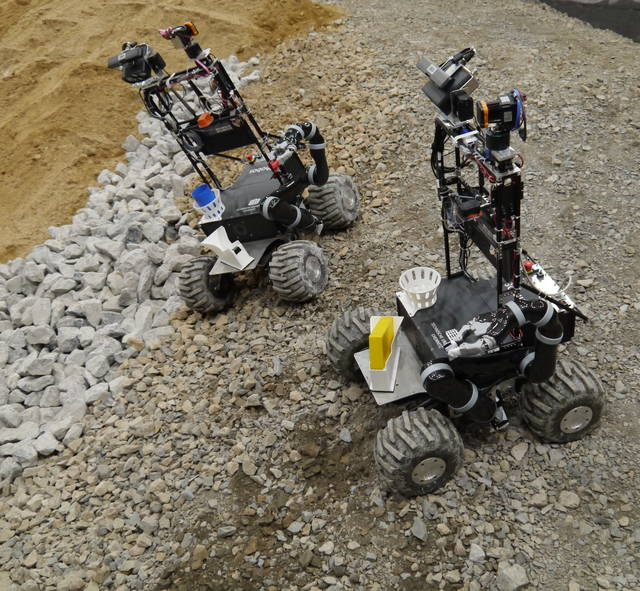
\includegraphics[width=0.75\textwidth]{beispiel.jpg}
  \caption{Die beiden Roboter Phobos und Deimos}
  \label{fig:roboter}
\end{figure}

Eine Referenz auf ein Bild wird wie folgt erzeugt: In Abbildung~\ref{fig:roboter} sind die beiden Roboter Phobos und Deimos dargestellt.

\section{Einbindung einer Tabelle}
Einbindung einer Tabelle:

\begin{table}[htb]
  \centering
  \begin{tabular}{l|c|r}
    Spalte 1 		& Spalte 2 	& Spalte 3 	\\
    linksbündig 	& zentriert 	& rechtsbündig 	\\
    1			& 2		& 3		\\
  \end{tabular}
  \caption{Eine Tabelle}
  \label{tab:table1}
\end{table}

Die Tabelle~\ref{tab:table1} ist nur ein minimales Beispiel.

\section{Angabe einer Literatur-Quelle}
Mehr Informationen über die Roboter der Professur Prozessautomatisierung können beispielsweise in \citep{robots} gefunden werden. Dazu müssen die Informationen zur Quelle im Bibtex-Style in die Datei \textit{literatur.bib} eingefügt werden.





%------- Literaturverzeichnis -------------------------------------------------------------------------
\newpage
\manualmark
\markboth{Literaturverzeichnis}{Literaturverzeichnis}
\printbibliography

%------- Anhang ----------------------------------------------------------------------------------------
\newpage
\appendix
\addcontentsline{toc}{chapter}{Anhang} % Zeigt ``Anhang'' in Inhaltsverzeichnis
\chapter{Daten-CD}	
\section{Digitale Version der Arbeit (PDF-Format)}
\section{Quellcode}
Beispiel Anhang. Hier die Funktionsweise des Quellcodes etc erklären.
\chapter{Ein weiterer Anhang}

%------- Selbstständigkeitserklärung --------------------------------------------------------------------
\chapter*{Selbstständigkeitserklärung}
Hiermit erkläre ich, dass ich die vorliegende Arbeit
selbstständig angefertigt, nicht anderweitig zu Prüfungszwecken vorgelegt und
keine anderen als die angegebenen Hilfsmittel verwendet habe. Sämtliche 
wissentlich verwendete Textausschnitte, Zitate oder Inhalte anderer Verfasser 
wurden ausdrücklich als solche gekennzeichnet.\bigskip\\
\dcplace, den \dcdate
\bigskip\bigskip
\flushleft
\newlength\us
\settowidth{\us}{-\dcfirstauthorfirstname~\dcfirstauthorlastname, \dcsecondauthorfirstname~\dcsecondauthorlastname-}
\begin{tabular}{p{\us}}\hline
\centering\footnotesize \dcfirstauthorfirstname~\dcfirstauthorlastname, \dcsecondauthorfirstname~\dcsecondauthorlastname
\end{tabular}

\end{document}

